\documentclass[11pt,a4paper]{article}
\usepackage[margin=25mm]{geometry}
\usepackage{graphicx,amsmath}
\title{Event 3790: origin and resolution of the arrival-time axis}
\date{\today}
\begin{document}\maketitle
For the single-electron sample, the saved event axis contains 502 buckets
and spans 0--10.04 s. It is a relative arrival-time axis,
\[
 t=(z-z_{\mathrm{first}})/v,\qquad v=0.1\ \mathrm{m/s}.
\]
The first longitudinal slice of the complete retained event defines zero.
The common absolute drift delay is not included. Individual pads use this same
axis, so charge reaching a late-arriving pad can appear after a long initial
interval of zero counts.

The source MC deposits extend from 540.8 to 1544.4 mm along z; the generation
vertex is at 1545.3 mm. Deposits separated by approximately one metre therefore
have approximately ten seconds of separation at this speed. 79.2\% of the
collected ions fall in the final second of the saved event interval. Earlier
charge belongs to other positions and pads. Only 15 of the 502
event buckets contain collected charge anywhere in the event.

The saved diffusion table has longitudinal cells 10.12 mm wide. The 20 ms
readout corresponds to 2 mm. Assigning the coarser diffusion-cell centres to
readout buckets can introduce artificial gaps and concentrate charge into
individual buckets. A finer diffusion-grid convergence check is required before
treating the derived event compression fractions as final. The circuit
calculation remains a response to the stored input counts.

\begin{figure}[ht]\centering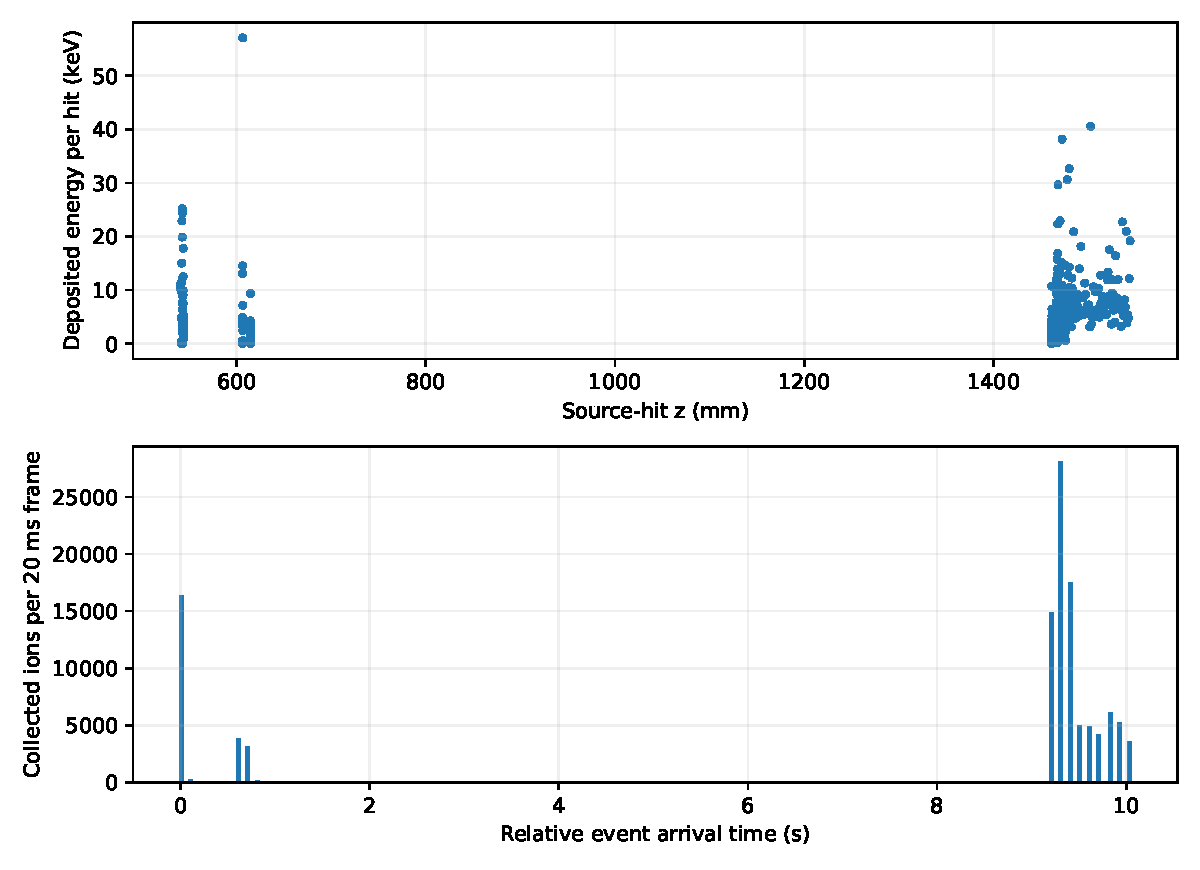
\includegraphics[width=\linewidth]{time_axis.pdf}
\caption{Source-hit longitudinal positions and the full collected-ion time
sequence for the single-electron event. The timing plot sums all pads.}
\end{figure}

The same numerical event ID in the double-beta sample is a different event;
its saved duration is 0.78 s. Input arrays, grid widths, fractions and
source hashes are saved in \texttt{results/ltspice/history\_time\_audit/}.
Reproduce from the repository root:
\begin{verbatim}
julia --project=. scripts/audit_history_time.jl 3790
python scripts/present_history_time_audit.py 3790
\end{verbatim}
The report source is generated without compiling a PDF.
\end{document}
